\documentclass[11pt]{ctexart}
\usepackage[margin=0.9in]{geometry}
\usepackage{graphicx}
\usepackage{booktabs}
\usepackage{amsmath}
\usepackage{float}
\usepackage{caption}
\usepackage[colorlinks=true,linkcolor=blue,citecolor=blue,urlcolor=blue]{hyperref}
\captionsetup{font=small,labelfont=bf}
\graphicspath{{../figures/}}
\newcommand{\NoisyPthree}{14.60}
\newcommand{\NoisySthree}{0.054}
\newcommand{\NoisyFthree}{10.73}
\newcommand{\DenPthree}{30.31}
\newcommand{\DenSthree}{0.835}
\newcommand{\DenFthree}{23.80}
\newcommand{\DecPthree}{31.34}
\newcommand{\DecSthree}{0.885}
\newcommand{\DecFthree}{24.61}
\newcommand{\UNetPthree}{32.27}
\newcommand{\UNetSthree}{0.907}
\newcommand{\UNetFthree}{25.25}
\newcommand{\NoisyPten}{19.53}
\newcommand{\NoisySten}{0.151}
\newcommand{\NoisyFten}{15.25}
\newcommand{\DenPten}{32.50}
\newcommand{\DenSten}{0.905}
\newcommand{\DenFten}{25.33}
\newcommand{\DecPten}{33.62}
\newcommand{\DecSten}{0.917}
\newcommand{\DecFten}{26.77}
\newcommand{\UNetPten}{34.74}
\newcommand{\UNetSten}{0.934}
\newcommand{\UNetFten}{27.68}
\newcommand{\NoisyPthirty}{24.10}
\newcommand{\NoisySthirty}{0.331}
\newcommand{\NoisyFthirty}{19.60}
\newcommand{\DenPthirty}{34.08}
\newcommand{\DenSthirty}{0.923}
\newcommand{\DenFthirty}{26.91}
\newcommand{\DecPthirty}{35.34}
\newcommand{\DecSthirty}{0.937}
\newcommand{\DecFthirty}{28.39}
\newcommand{\UNetPthirty}{36.70}
\newcommand{\UNetSthirty}{0.950}
\newcommand{\UNetFthirty}{29.67}
\newcommand{\NoisyPonehundred}{28.81}
\newcommand{\NoisySonehundred}{0.596}
\newcommand{\NoisyFonehundred}{23.92}
\newcommand{\DenPonehundred}{35.36}
\newcommand{\DenSonehundred}{0.935}
\newcommand{\DenFonehundred}{28.22}
\newcommand{\DecPonehundred}{37.16}
\newcommand{\DecSonehundred}{0.952}
\newcommand{\DecFonehundred}{30.22}
\newcommand{\UNetPonehundred}{38.61}
\newcommand{\UNetSonehundred}{0.963}
\newcommand{\UNetFonehundred}{31.63}
\newcommand{\NoisyPthreehundred}{32.48}
\newcommand{\NoisySthreehundred}{0.793}
\newcommand{\NoisyFthreehundred}{26.95}
\newcommand{\DenPthreehundred}{36.26}
\newcommand{\DenSthreehundred}{0.947}
\newcommand{\DenFthreehundred}{29.01}
\newcommand{\DecPthreehundred}{38.63}
\newcommand{\DecSthreehundred}{0.963}
\newcommand{\DecFthreehundred}{31.67}
\newcommand{\UNetPthreehundred}{40.01}
\newcommand{\UNetSthreehundred}{0.971}
\newcommand{\UNetFthreehundred}{33.03}
\newcommand{\DecGainThree}{0.93}
\newcommand{\DecCIThree}{0.83--1.05}
\newcommand{\DecGainTen}{1.12}
\newcommand{\DecCITen}{1.06--1.19}
\newcommand{\DecGainThirty}{1.36}
\newcommand{\DecCIThirty}{1.23--1.49}
\newcommand{\DecGainHundred}{1.45}
\newcommand{\DecCIHundred}{1.34--1.57}
\newcommand{\DecGainThreeHundred}{1.37}
\newcommand{\DecCIThreeHundred}{1.25--1.51}
\newcommand{\DenGainThree}{1.96}
\newcommand{\BestGainThree}{0.93}
\newcommand{\BestGainThirty}{1.36}
\newcommand{\BestGainThreeHundred}{1.37}
\newcommand{\BestGainMin}{0.93}
\newcommand{\BestGainMax}{1.45}
\newcommand{\PSNRThirtyTwoDec}{30}
\newcommand{\PSNRThirtyTwoU}{10}
\newcommand{\PSNRThirtyTwoFactor}{3.0}
\newcommand{\SSIMNineDec}{30}
\newcommand{\SSIMNineU}{10}
\newcommand{\SSIMNineFactor}{3.0}
\newcommand{\SSIMNineTwoDec}{30}
\newcommand{\SSIMNineTwoU}{30}
\newcommand{\SSIMNineTwoFactor}{1.0}
\newcommand{\FGTwoSixDec}{100}
\newcommand{\FGTwoSixU}{30}
\newcommand{\FGTwoSixFactor}{3.3}
\newcommand{\CrossDecFourteen}{1.36}
\newcommand{\CrossDecFifteen}{0.52}
\newcommand{\CrossDecSixteen}{1.30}
\newcommand{\CrossDecEighteen}{0.16}
\newcommand{\CrossDecMin}{0.16}
\newcommand{\CrossDecMax}{1.30}
\newcommand{\SpecPthree}{32.36}
\newcommand{\SpecSthree}{0.908}
\newcommand{\SpecFthree}{25.32}
\newcommand{\SpecPthirty}{36.72}
\newcommand{\SpecSthirty}{0.951}
\newcommand{\SpecFthirty}{29.67}
\newcommand{\SpecPonehundred}{38.68}
\newcommand{\SpecSonehundred}{0.963}
\newcommand{\SpecFonehundred}{31.74}
\newcommand{\CondPthree}{32.20}
\newcommand{\CondSthree}{0.905}
\newcommand{\CondFthree}{25.17}
\newcommand{\CondPthirty}{36.44}
\newcommand{\CondSthirty}{0.948}
\newcommand{\CondFthirty}{29.34}
\newcommand{\CondPonehundred}{38.29}
\newcommand{\CondSonehundred}{0.961}
\newcommand{\CondFonehundred}{31.27}
\newcommand{\BlindPthree}{32.27}
\newcommand{\BlindSthree}{0.907}
\newcommand{\BlindFthree}{25.25}
\newcommand{\ScrPthree}{30.19}
\newcommand{\BlindPthirty}{36.70}
\newcommand{\BlindSthirty}{0.950}
\newcommand{\BlindFthirty}{29.67}
\newcommand{\ScrPthirty}{34.46}
\newcommand{\BlindPonehundred}{38.61}
\newcommand{\BlindSonehundred}{0.963}
\newcommand{\BlindFonehundred}{31.63}
\newcommand{\ScrPonehundred}{36.18}
\newcommand{\CondDeltaLow}{-0.33}
\newcommand{\CondDeltaHigh}{-0.07}
\newcommand{\CondStrongPthree}{32.29}
\newcommand{\CondStrongPthirty}{36.71}
\newcommand{\CondStrongPonehundred}{38.66}
\newcommand{\CondStrongLow}{+0.01}
\newcommand{\CondStrongHigh}{+0.05}
\newcommand{\CondStrongDelta}{0.05}
\newcommand{\AucThree}{0.96}
\newcommand{\AucTen}{0.96}
\newcommand{\NFailThirty}{1}
\newcommand{\RhoThree}{0.92}
\newcommand{\SigmaUPfifteen}{36.92}
\newcommand{\SigmaDecfifteen}{35.85}
\newcommand{\SigmaUPtwo}{36.70}
\newcommand{\SigmaDectwo}{35.34}
\newcommand{\SigmaUPtwopfive}{35.76}
\newcommand{\SigmaDectwopfive}{34.76}
\newcommand{\AiryStrongUThree}{32.63}
\newcommand{\AiryStrongGainThree}{+1.42}
\newcommand{\AiryStrongUThirty}{36.64}
\newcommand{\AiryStrongGainThirty}{+0.41}
\newcommand{\AiryStrongUThreeHundred}{37.05}
\newcommand{\AiryStrongGainThreeHundred}{-3.21}
\newcommand{\AiryUThree}{32.71}
\newcommand{\AiryTvThree}{31.21}
\newcommand{\AiryGainThree}{1.50}
\newcommand{\AiryCIThree}{1.35--1.65}
\newcommand{\AiryUThirty}{37.61}
\newcommand{\AiryTvThirty}{36.23}
\newcommand{\AiryGainThirty}{1.39}
\newcommand{\AiryCIThirty}{1.28--1.48}
\newcommand{\AiryUThreeHundred}{41.55}
\newcommand{\AiryTvThreeHundred}{40.26}
\newcommand{\AiryGainThreeHundred}{1.29}
\newcommand{\AiryCIThreeHundred}{1.13--1.45}
\newcommand{\PsfMixGaussPThree}{32.26}
\newcommand{\PsfMixGaussPThirty}{36.60}
\newcommand{\PsfMixGaussPThreeHundred}{39.83}
\newcommand{\HeldoutPFive}{33.32}
\newcommand{\HeldoutPFifty}{37.50}
\newcommand{\HeldoutPTwoHundred}{39.47}
\newcommand{\HeldoutResFive}{0.00}
\newcommand{\HeldoutResFifty}{0.01}
\newcommand{\HeldoutResTwoHundred}{0.02}
\newcommand{\SpeedCPU}{29.3}
\newcommand{\SpeedGPU}{1.2}
\newcommand{\SpeedTV}{103}
\newcommand{\SpeedFactorCPU}{3.5}
\newcommand{\SpeedFactorGPU}{86}

\newcommand{\RealN}{243}
\newcommand{\RealNoisyP}{16.44}
\newcommand{\RealNoisyS}{0.107}
\newcommand{\RealBMThreeP}{24.83}
\newcommand{\RealBMThreeS}{0.559}
\newcommand{\RealNlmP}{24.78}
\newcommand{\RealNlmS}{0.551}
\newcommand{\RealTvP}{24.51}
\newcommand{\RealTvS}{0.526}
\newcommand{\RealUnetP}{29.01}
\newcommand{\RealUnetS}{0.877}
\newcommand{\RealBMThreeRawP}{21.30}
\newcommand{\RealBMThreeRawS}{0.359}
\newcommand{\RealNlmRawP}{21.28}
\newcommand{\RealNlmRawS}{0.354}
\newcommand{\RealTvRawP}{20.58}
\newcommand{\RealTvRawS}{0.333}
\newcommand{\RealGain}{4.18}
\newcommand{\RealGainRaw}{7.70}
\newcommand{\RealCI}{3.94--4.42}
\newcommand{\RealGainNlm}{4.23}
\newcommand{\RealGainTv}{4.50}
\newcommand{\RealWins}{240}
\newcommand{\RealPvalue}{2.2e-41}
\newcommand{\RealBmSigma}{0.3}
\newcommand{\RealNlmH}{0.2}
\newcommand{\RealTvW}{0.24}
\newcommand{\RealDncnnP}{28.80}
\newcommand{\RealDncnnS}{0.865}
\newcommand{\RealDncnnGain}{3.97}
\newcommand{\RealUnetGainDncnn}{0.21}
\newcommand{\RealUnetDncnnCI}{0.15--0.28}
\newcommand{\RealUnetDncnnWins}{210}
\newcommand{\LargeRealN}{20}
\newcommand{\LargeRealNoisyP}{13.35}
\newcommand{\LargeRealBMThreeP}{17.05}
\newcommand{\LargeRealNlmP}{16.89}
\newcommand{\LargeRealTvP}{16.45}
\newcommand{\LargeRealUnetP}{15.83}

\newcommand{\FmdN}{150}
\newcommand{\FmdNoisyP}{25.62}
\newcommand{\FmdNoisyS}{0.584}
\newcommand{\FmdBMThreeP}{28.07}
\newcommand{\FmdBMThreeS}{0.704}
\newcommand{\FmdNlmP}{26.96}
\newcommand{\FmdNlmS}{0.697}
\newcommand{\FmdTvP}{27.01}
\newcommand{\FmdTvS}{0.707}
\newcommand{\FmdUnetP}{31.74}
\newcommand{\FmdUnetS}{0.845}
\newcommand{\FmdGain}{3.67}
\newcommand{\FmdWins}{147}
\newcommand{\FmdPvalue}{2.9e-26}
\newcommand{\FmdCI}{3.27--4.12}
\newcommand{\FmdStrataMin}{0.4}
\newcommand{\FmdStrataMax}{11.1}
\newcommand{\FmdStrataN}{36}

\title{\bfseries 面向低剂量荧光显微的\\剂量无关神经反卷积}
\author{}
\date{\today}
\begin{document}
\maketitle

\begin{abstract}
荧光显微受光子预算限制：提高信噪比的光同时会加速光漂白和光毒性。计算恢复可以从较少光子中重建结构，但在一个噪声水平有效的正则化强度，换一个剂量往往失效；多数学习模型又只针对窄剂量范围训练或条件化。实际采集时光子数往往未知、随视野变化并随设置改变，逐剂量重调难以部署。本文要问：一个模型能否在不需要剂量元数据的情况下覆盖宽剂量范围，以及相对调好的经典方法能节省多少光子预算。

我们在 100 倍剂量范围上训练单个混合剂量 U-Net，推理时不输入光子数，并与逐剂量调参的 TV-ADMM 反卷积比较。为了让比较可操作，我们在验证视野上按目标成功率选择剂量，再原样应用到 held-out 视野。该模型在整个范围上比调好的 TV-ADMM 高 \BestGainMin--\BestGainMax\,dB，在匹配 90\% 成功率时把光子预算降至约 1/3（3--3.3 倍节省）；在真实噪声/干净对上（去噪检查）比 affine 校准 BM3D 高 \RealGain\,dB。对照实验表明增益来自学到的样本结构而非容量，PSF 混合变体在 Airy PSF 下仍保持增益。剂量扫描是模拟的，真实增益是同源的；两者共同说明一个模型可以替代逐剂量调参，恢复方法应在匹配成功率下比较。
\end{abstract}

\noindent\textbf{关键词：}荧光显微；反卷积；低剂量成像；深度学习；剂量无关恢复；不确定度

\section{引言}
荧光显微本质上受探测光子数限制。提高激发功率或曝光时间可以改善信噪比，但也会加速光漂白和光毒性，对活细胞尤其不利\cite{laissue2017phototoxicity}。计算恢复提供了一条出路：从已经采集到的光子中尽可能恢复结构。反卷积在抑制散粒噪声的同时去除衍射极限点扩散函数（PSF），但随着光子数下降，逆问题越来越病态。在某个剂量下能保留细节的正则化强度，在更低剂量下会放大噪声；而在低剂量下能压噪声的强度，在更高剂量下又会抹掉结构。

经典反卷积把这一权衡显式化。Richardson--Lucy\cite{richardson1972,lucy1974}、Wiener 滤波\cite{wiener1949}、全变分\cite{chambolle2004,rudin1992}、非局部均值\cite{buades2005}以及盲反卷积\cite{kundur1996}都依赖噪声模型和一个需要针对特定信号水平选择的权重；综述见\cite{wallace2001}。深度学习用成对图像学到的先验替代手工先验。CARE\cite{weigert2018care}及其部署工具\cite{gomez2021deepimagej}让 U-Net 恢复成为常规手段，监督恢复也被推广到跨模态超分辨\cite{wang2019crossmodality}。在去噪中，噪声水平条件化是标准做法\cite{zhang2018ffdnet}；盲去噪器可以估计噪声水平或无需显式噪声水平\cite{guo2019cbdnet,mohan2020biasfree,krull2019}，但这些方法做的是去噪而不是反卷积，也没有在匹配成功率下跨宽剂量范围评估。基于模型的深度反卷积\cite{liu2020degeneration}、零样本反卷积\cite{qiao2024zsdeconvnet}、不确定度驱动的自适应扫描\cite{ye2025uncertainty}和近零光子成像\cite{sheneman2025nearzero}分别解决了问题的不同部分。然而在显微中，每像素光子数往往未知、随视野变化，并随采集设置改变；逐剂量重调或重训只在很窄的范围内可行。低剂量成像真正要问的是：一个模型能否在不知道剂量的情况下覆盖宽剂量范围，以及相对一个调好的经典方法究竟能省多少光子预算。本文的贡献不是新的网络结构，而是对这个问题做受控检验，并在匹配成功率而非单一剂量下量化光子节省。

我们在公开显微图像上做一个受控研究。一个 U-Net 在覆盖 100 倍剂量范围的图像块上训练；网络只接收含噪图像，没有剂量通道，因此必须从数据中推断局部噪声水平。我们与已知 PSF 的 TV 反卷积、TV 去噪、Wiener 滤波和 Richardson--Lucy 比较，所有基线都逐剂量在验证集上调参；NLM 也纳入定性和扩展比较。数据按视野（FOV）切分，测试 FOV 从不用于训练、调参或早停。为了让比较可操作，我们定义协议准则：在验证 FOV 上选择达到 90\% 成功的最小剂量，然后原样应用到 held-out FOV；这避免了在测试集上选工作点，也把剂量响应曲线变成光子预算比较。

在这个范围上，盲模型在每个剂量都优于调好的 TV-ADMM，提升 \BestGainMin--\BestGainMax\,dB；匹配 90\% 成功时，只需约 1/3 的光子预算（3--3.3 倍节省）。它还能迁移到三个 held-out 染色数据，增益较小。真实数据检查的是去噪：在同源协议上重新训练后，网络相对 affine 校准 BM3D 提升 \RealGain\,dB，预算匹配的 DnCNN 紧随其后。对照实验区分了增益来源：同预算的相位打乱网络低于 TV，而剂量条件化和逐剂量专家带来的提升很小，说明增益不能由容量或元数据解释；PSF 混合变体在物理 Airy PSF 下仍保持增益，而只在高斯核上训练的模型在高剂量下失去优势（SI S4d）。

在实践上，这去掉了一个校准维度。活细胞成像可接受的光子剂量由样品决定，而不是由恢复算法决定；一个覆盖整个范围、不需要元数据的模型可以训练一次并随协议复用，协议曲线则给出达到目标质量所需的剂量。它也改变了方法比较方式：在某个剂量上测到的增益，换一个剂量可能变大或变小，真正有意义的是匹配成功率下所需的光子预算。本文的范围有两点限制：剂量扫描是用已知高斯 PSF 和 Poisson 噪声模拟的；真实成对数据只在同一采集协议内检验恢复，同一组权重不能零样本迁移到另一个来源。在这个范围内，结果支持剂量无关恢复。

\section{方法}
\paragraph{前向模型。}
干净 FOV $x$ 先被宽度为 $\sigma$ 的高斯 PSF 模糊，再受 Poisson 散粒噪声污染：
\begin{equation}
y=\frac{1}{P}\operatorname{Poisson}\!\left(P\,(g_\sigma * x)\right),
\label{eq:forward}
\end{equation}
其中 $P$ 是全幅 Poisson 尺度：归一化强度为 $x$ 的像素，其期望探测光子数为 $Px$。除非特别说明，$\sigma=2$ 像素，$P$ 取 3--300 全幅单位；测试块上的平均探测光子数分别为 0.36、3.56、35.6（$P=3,30,300$，\texttt{results/photon\_units.json}）。由于期望光子数随 $P$ 线性变化，$P$ 的比值也是光子预算的比值。经典基线使用与生成数据相同的 PSF。

\paragraph{数据。}
我们使用 Broad Bioimage Benchmark Collection 的四个公开数据集\cite{ljosa2012bbbc}。主数据集是 BBBC014 channel~1（96 个 FOV，$1360\times1024$，8-bit，CC BY 3.0），按 FOV 切成 56 个训练、20 个验证、20 个测试。验证 FOV 用于早停和所有经典基线的调参；测试 FOV 不参与训练、调参或模型选择。BBBC015、BBBC016（U2OS 胞质-核实验，CC BY 3.0）和 BBBC018（actin 通道，不同细胞类型和染色，CC BY-NC-SA 3.0）只作为外部测试集，各均匀取 20 个 FOV（5 个用于 TV 调参，15 个 held-out 评估），图像按 8-bit 满量程归一化。

\paragraph{真实噪声/干净数据。}
真实噪声检查使用公开 AI4Life-MDC25-Nuclei\cite{ai4life_mdc25_2025}（Zenodo 15624741，CC BY 4.0），即 2025 AI4Life 显微监督去噪挑战的训练集。它包含 2{,}457 对 $256\times256$ 的 Jacquemet 噪声细胞核图像和 20 对 $1024\times1024$ 的 BBBC006 图像；两个来源在位深、饱和和噪声模型上不同。为谨慎起见，我们排除与大幅场 ID 数字重合的 20 个小图 ID（图像本身不是彼此的裁剪），余下 2{,}437 对按图像 ID 切成 1{,}951 个训练、243 个验证、243 个测试。没有场共享：在全部 1{,}951 张训练图上，测试-训练缩略图最大相关为 0.55，没有一对超过 0.8，最高一对的全分辨率相关为 0.06（\texttt{results/real\_leakage\_full.json}）。真实比较使用全部 \RealN\ 个 held-out 对；经典输出在验证对上做 affine 校准。20 个大幅 BBBC006 对不参与训练或调参，只用于跨来源检查。

\paragraph{第二个真实来源。}
FMD 数据\cite{zhang2019fmd,ai4life_mdc25_fmd_2025}（Zenodo 15761900，CC BY 4.0）包含来自三台显微镜、三个通道、四个噪声水平的 63{,}669 对 $256\times256$ 噪声/干净图像。我们按 field 取每场一帧（seed 0），按 field 分层切成 1{,}396/301/301 训练/验证/测试，没有一帧跨 split。主比较使用预先指定的 150 个 held-out field：每个 microscope/channel/level 层按 field ID 字典序取前 4 个，再从字典序前 6 层各补第 5 个；选择规则写在 \texttt{prereg/fmd\_subset150.json}，在任何模型预测前固定。

\paragraph{网络与训练。}
网络是三级 U-Net\cite{ronneberger2015unet}，通道数为 64、128、256，$3\times3$ 卷积。训练块为 $64\times64$，从训练 FOV 随机裁剪，并做随机翻转和 $90^\circ$ 旋转。主混合剂量模型对每个块从 $\{3,10,30,100,300\}$ 全幅单位中采样剂量，只接收含噪图像，训练和推理都不使用剂量通道。它使用 48{,}000 个 patch、150 个 epoch，按所有剂量平均的验证 PSNR 早停；优化器为 Adam，学习率 $10^{-3}$，余弦 schedule，损失为均方误差。PSF 鲁棒变体使用相同 schedule，但每个训练块随机用高斯（$\sigma=2$）或标量 Airy PSF（NA 1.4，$\lambda=520$\,nm，100\,nm 像素）模糊。基预算消融使用 32 通道条件化变体（24{,}000 patch、100 epoch）；预算匹配条件化模型重复完整的 64 通道/48k/150 设置。条件化变体增加一个常数剂量通道 $c(P)=(\log_{10}P-\log_{10}3)/(\log_{10}300-\log_{10}3)$。逐剂量专家使用同样的 64 通道/48k/150 设置，分别在 3、30、100 全幅单位训练。两个相位打乱对照把每个训练 FOV 替换为同功率谱的随机相位替代，同时保持验证/测试 FOV 不变：一个基预算对照（32 通道、24k patch、100 epoch）和一个预算匹配盲对照（64 通道、48k patch、150 epoch、混合剂量）。验证使用每个 FOV 4 个分散的 $128\times128$ patch。

\paragraph{真实数据模型。}
真实数据网络是 CARE 式监督 U-Net（与模拟模型相同的三级编码器-解码器，第一级 48 通道），在真实训练对的 $128\times128$ patch 上训练（16{,}000 patch、80 epoch、batch 64、Adam、学习率 $10^{-3}$、余弦 schedule），并做翻转和 $90^\circ$ 旋转。每张图独立归一化到 0.5--99.9 百分位。验证在 243 个 held-out 小对上选择 checkpoint（28.6\,dB）。对细胞核对，经典基线在 5 个验证对上用扩展网格调参（BM3D\cite{dabov2007} $\sigma\in[0.2,1.0]$、NLM $h\in[0.1,0.3]$、TV 权重 $\in[0.08,0.4]$），选定值为 $\sigma=\RealBmSigma$、$h=\RealNlmH$、$w=\RealTvW$。每个经典输出再用一个在验证对上拟合的全局 affine 变换（增益和偏置）映射；原始未校准值放在 SI。第二个监督基线是 17 层 DnCNN\cite{zhang2017dncnn}，64 通道、残差噪声预测，使用相同的 16{,}000 patch 和 80 epoch、相同归一化和增广（验证 28.2\,dB）。FMD 模型使用较小的基预算（32 通道、8{,}000 patch、40 epoch），因此是次要检查；其经典基线按显微镜分别在 5 个验证场上调参：BM3D $\sigma$ 为 0.12（CF）、0.15（TP）、8.0（WF，WF 网格扩到 20 以避免边界解），NLM $h=0.1$，TV 权重 0.08（CF）/0.12（TP,WF）。FMD checkpoint 在 60 个 FMD 验证场上选择。测试对不用于调参或早停。

\paragraph{基线。}
主要经典基线是 TV 正则反卷积：求解 $\min_x \tfrac12\|Hx-y\|^2+\lambda\,\mathrm{TV}(x)$，使用 ADMM\cite{boyd2011}、已知 PSF $H$ 和 30 次迭代。TV 权重 $\lambda$ 和 ADMM 惩罚 $\rho$ 都在 5 个验证 FOV（50 个 patch）上逐剂量调参，边界用 reflect padding。我们还报告不做去模糊的 TV 去噪（在 $y$ 上做 Chambolle TV）、Wiener 滤波和同 PSF 的 Richardson--Lucy。NLM 在 Anscombe 方差稳定变换\cite{anscombe1948,makitalo2011}后使用；Wiener、Richardson--Lucy 的扩展网格放在 SI。所有经典参数都在与网络相同剂量和 PSF 的验证 FOV 上调参。

\paragraph{指标与统计。}
我们报告 PSNR、SSIM\cite{wang2004ssim}和前景 PSNR（真值强度前 10\%）。主比较和协议使用每个 FOV 10 个分散的 $128\times128$ patch，先按 FOV 聚合。协议剂量是 $\{3,10,30,100,300\}$ 全幅单位中，使至少 90\% 验证 FOV 达到目标的最小剂量，然后原样用于测试 FOV；test-oracle 剂量只作为上界放在 SI。90\% 对应 18/20 个 FOV，五点网格使报告的因子是离散的。比较使用逐 FOV 配对差、FOV bootstrap 95\% 置信区间和精确 Wilcoxon 符号秩检验；$n=20$。只有 FOV 检验和置信区间一致时才报告效应。

\paragraph{不确定度。}
我们按 deep ensemble\cite{lakshminarayanan2017ensembles}训练三个不同随机种子的剂量条件化网络。给定剂量，三个预测的逐像素标准差作为不确定度图，其 FOV 均值作为不确定度分数。不确定度分析使用条件化变体作为混合剂量模型的代理。我们用 PSNR 低于 34\,dB 的 FOV 做失败检测的 ROC AUC，并计算与重建 RMSE 的秩相关；30 光子时只有一个 FOV 低于目标，因此不报告该剂量的 AUC。

\paragraph{计时。}
在 NVIDIA A100 GPU 上测网络单 patch 推理时间，在单 CPU 核上测 30 次 ADMM 迭代的 TV 反卷积时间；网络也在单 CPU 核上计时以做同硬件比较。

\section{结果}
\subsection{公平反卷积比较}
表~\ref{tab:perf} 给出五个剂量，图~\ref{fig:quant} 展示 $P=3,10,30$ 的重建。$P=3$ 时混合剂量网络达到 \UNetPthree\,dB PSNR 和 \UNetSthree\ SSIM，对比调好的 TV 反卷积 \DecPthree\,dB/\DecSthree、TV 去噪 \DenPthree\,dB/\DenSthree、噪声输入 \NoisyPthree\,dB；前景 PSNR 为 \UNetFthree\,dB，对比 TV 反卷积 \DecFthree\,dB。优势在每个剂量都存在：30 光子时网络 \UNetPthirty\,dB 对 \DecPthirty\,dB，300 光子时 \UNetPthreehundred\,dB 对 \DecPthreehundred\,dB。逐 FOV 配对差在 $P=3,10,30,100,300$ 分别为 \DecGainThree\,dB（95\% CI \DecCIThree）、\DecGainTen\,dB（\DecCITen）、\DecGainThirty\,dB（\DecCIThirty）、\DecGainHundred\,dB（\DecCIHundred）、\DecGainThreeHundred\,dB（\DecCIThreeHundred）；每个剂量都在全部 20 个测试 FOV 上获胜（Wilcoxon $p<10^{-5}$）。SSIM 从 $P=3$ 的 \DecSthree\ 提升到 \UNetSthree，从 $P=300$ 的 \DecSthreehundred\ 提升到 \UNetSthreehundred。

\begin{table}[H]
\centering
\caption{20 个 held-out BBBC014 FOV 上的重建（每 FOV 10 个 $128\times128$ patch）。PSNR（dB）、SSIM 和前景 PSNR（dB）。U-Net 为无剂量输入的混合剂量模型；TV 反卷积为已知 PSF 的 ADMM，TV 去噪为不做去模糊的 Chambolle TV。经典参数在每个剂量的验证 FOV 上调参。}
\label{tab:perf}
\begin{tabular}{lcccc}
\toprule
 & 噪声输入 & TV 去噪 & TV 反卷积 & U-Net \\
\midrule
\multicolumn{5}{l}{\emph{$P=3$ (全幅单位)}} \\
PSNR（dB） & 14.60 & 30.31 & 31.34 & 32.27 \\
SSIM & 0.054 & 0.835 & 0.885 & 0.907 \\
前景 PSNR（dB） & 10.73 & 23.80 & 24.61 & 25.25 \\
\midrule
\multicolumn{5}{l}{\emph{$P=10$ (全幅单位)}} \\
PSNR（dB） & 19.53 & 32.50 & 33.62 & 34.74 \\
SSIM & 0.151 & 0.905 & 0.917 & 0.934 \\
前景 PSNR（dB） & 15.25 & 25.33 & 26.77 & 27.68 \\
\midrule
\multicolumn{5}{l}{\emph{$P=30$ (全幅单位)}} \\
PSNR（dB） & 24.10 & 34.08 & 35.34 & 36.70 \\
SSIM & 0.331 & 0.923 & 0.937 & 0.950 \\
前景 PSNR（dB） & 19.60 & 26.91 & 28.39 & 29.67 \\
\midrule
\multicolumn{5}{l}{\emph{$P=100$ (全幅单位)}} \\
PSNR（dB） & 28.81 & 35.36 & 37.16 & 38.61 \\
SSIM & 0.596 & 0.935 & 0.952 & 0.963 \\
前景 PSNR（dB） & 23.92 & 28.22 & 30.22 & 31.63 \\
\midrule
\multicolumn{5}{l}{\emph{$P=300$ (全幅单位)}} \\
PSNR（dB） & 32.48 & 36.26 & 38.63 & 40.01 \\
SSIM & 0.793 & 0.947 & 0.963 & 0.971 \\
前景 PSNR（dB） & 26.95 & 29.01 & 31.67 & 33.03 \\
\bottomrule
\end{tabular}

\end{table}

\begin{figure}[H]
\centering
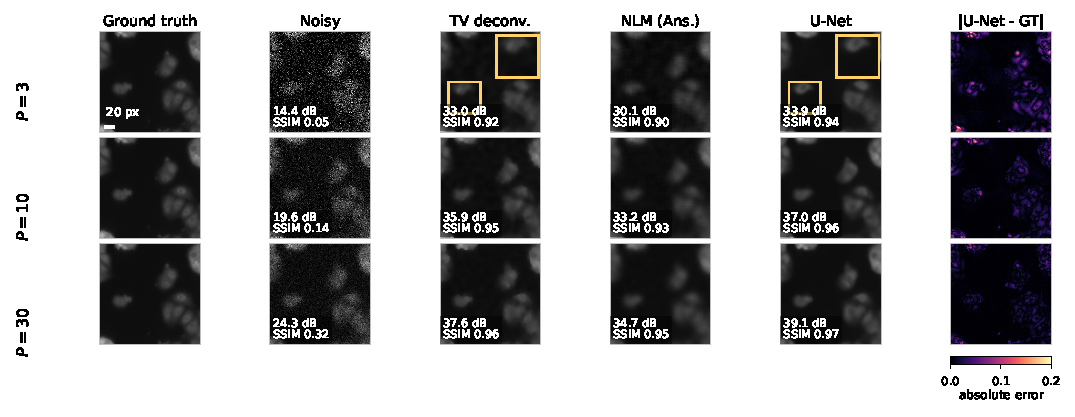
\includegraphics[width=\linewidth]{fig1_qualitative.pdf}
\caption{$P=3,10,30$ 时的定性重建，固定 $192\times192$ 测试裁剪（seed 7，不按性能挑选）。列为真值、噪声输入、TV 反卷积、NLM、混合剂量 U-Net 和 U-Net 绝对误差。比例尺 20 像素；公开 BBBC014 数据没有像素尺寸标定，因此不声称物理单位。所有图像使用相同的 $[0,1]$ 归一化强度。黄框和插图放大 TV 与 U-Net 面板中同一 $60\times60$ 区域（约 1.3 倍）。面板 PSNR 是这一裁剪的值，不是表~\ref{tab:perf} 的 FOV 均值。网络恢复了 TV 反卷积抹掉的边界和内部纹理，误差集中在边缘。}
\label{fig:quant}
\end{figure}

TV 反卷积在每个剂量都是最强的经典方法；不做去模糊的 TV 去噪在 3 光子时比网络低 \DenGainThree\,dB，而公平 TV 反卷积低 \DecGainThree\,dB。相对 TV 反卷积的增益在 3、30、300 光子分别为 \DecGainThree、\DecGainThirty、\DecGainThreeHundred\,dB，没有单调剂量趋势；最大在 $P=100$（1.45\,dB），最小在 $P=3$（0.93\,dB）。

\subsection{匹配质量所需光子剂量}
图~\ref{fig:dose}a--c 给出 PSNR、SSIM、前景 PSNR 随剂量的变化。图~\ref{fig:dose}e 把曲线转成固定协议：在 20 个验证 FOV 上选择达到 90\% 成功的最小剂量，再原样用于测试 FOV。PSNR 32\,dB 时 TV 反卷积需要 30 光子、网络 10（$3\times$）；PSNR 34\,dB 时 TV 需要 100、网络 30（$3.3\times$）。SSIM 0.90 时 TV 30、网络 10（$3\times$）；SSIM 0.85 和 0.92 都是平局（分别 3 和 30）。前景 PSNR 26\,dB 时 TV 100、网络 30（$3.3\times$）；24\,dB 时都是 10（平局）。PSNR 30\,dB 和前景 PSNR 22\,dB 处，验证集选出的剂量在测试集只达到 80\%，因此不声称因子（SI S2b）。支持的节省是四项 3--3.3 倍、三项平局；如果在测试集上选剂量，上界是五项 3--3.3 倍、四项平局。因子是离散的，20 个 FOV 样本也小；test-oracle bootstrap 的逐目标 CI 在 SI S2b，PSNR 32\,dB 处 96.6\% 的重采样至少给出 $3\times$。模型也不局限于五个训练剂量：在未参与训练的 $P=5,50,200$，它分别达到 \HeldoutPFive、\HeldoutPFifty、\HeldoutPTwoHundred\,dB，与相邻训练剂量的对数插值相差不超过 0.02\,dB（SI S4c）。

\begin{figure}[H]
\centering
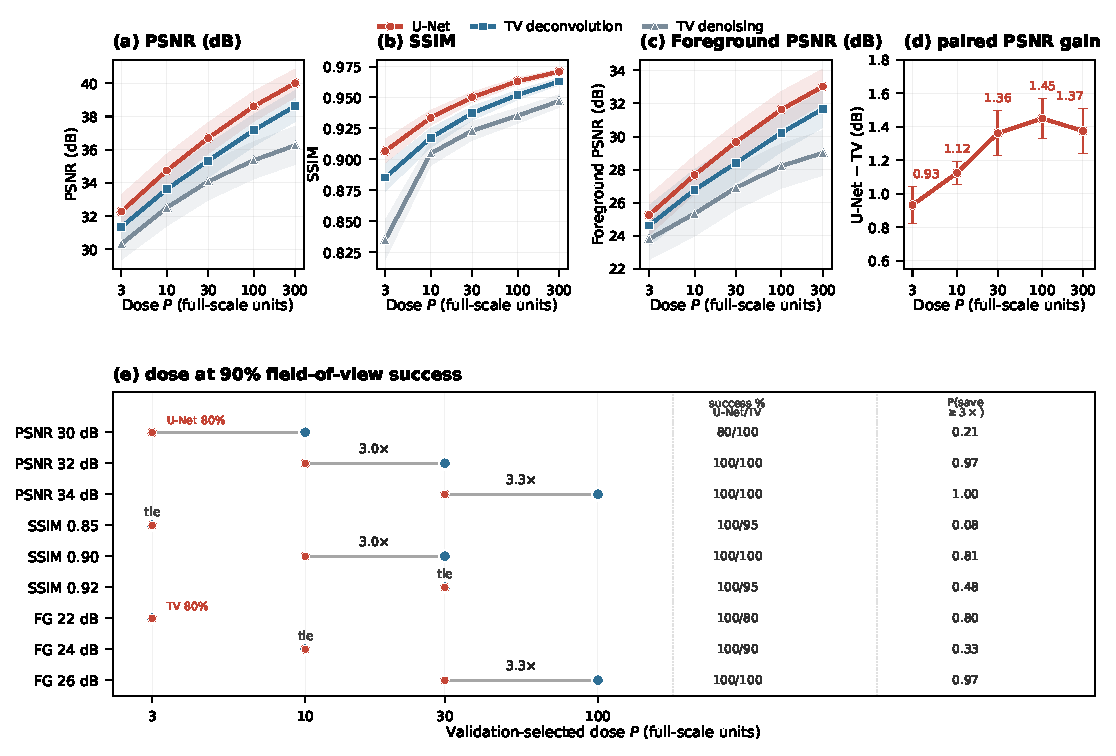
\includegraphics[width=\linewidth]{fig2_dose_response.pdf}
\caption{(a--c) 20 个 held-out FOV 上 PSNR、SSIM、前景 PSNR 随剂量 $P$ 的变化，阴影为 95\% 置信区间。(d) U-Net 相对 TV 反卷积的配对 PSNR 增益，误差棒为 95\% 置信区间。(e) 在验证 FOV 上选出的 90\% 成功剂量；蓝点为 TV 反卷积，红点为 U-Net。只有当两种方法在 held-out FOV 上也达到 90\% 时才显示因子；“tie” 表示同剂量，标签表示验证集选出的剂量在测试集只到 80\% 的方法。右侧文字列给出 held-out 成功率（U-Net/TV，\%）和 bootstrap 概率 P(节省 $\geq3\times$)。test-oracle 剂量和 bootstrap CI 在 SI S2b。}
\label{fig:dose}
\end{figure}

我们也比较了混合剂量模型、剂量条件化变体和逐剂量专家。预算匹配的条件化变体（64 通道、48k patch、150 epoch）在 $P=3,30,100$ 达到 \CondStrongPthree、\CondStrongPthirty、\CondStrongPonehundred\,dB，对比盲模型 \BlindPthree、\BlindPthirty、\BlindPonehundred\,dB；两者相差 \CondStrongDelta\,dB（\CondStrongLow--\CondStrongHigh），但前者推理时需要光子数。逐剂量专家使用同样的 64 通道/48k/150 预算，在自己剂量上达到 \SpecPthree、\SpecPthirty、\SpecPonehundred\,dB，与盲模型相差 0.1\,dB，但每个剂量需要一个模型和剂量标签。因此更简单的盲模型更可取：它与条件化变体相差 0.05\,dB，与专家相差 0.1\,dB，却不需要任何采集元数据。

\subsection{跨细胞类型和染色}
在 BBBC014 channel~1 上训练的模型不做重训就迁移到三个形态和染色不同的 held-out 数据集（图~\ref{fig:cross}a、表~\ref{tab:cross}）。30 光子时，它在 BBBC015 上比调好的 TV 反卷积高 \CrossDecFifteen\,dB、BBBC016 高 \CrossDecSixteen\,dB、BBBC018 高 \CrossDecEighteen\,dB；域内增益为 \CrossDecFourteen\,dB。外部置信区间不含零，但增益比域内小，BBBC018 的增益很有限；迁移是正向的，但不能替代域内训练。

\begin{table}[H]
\centering
\caption{30 光子时的跨数据集 PSNR。BBBC014 用 20 个测试 FOV；每个外部数据集分成 5 个验证 field 调 TV、15 个 held-out field 评估。模型只在 BBBC014 channel~1 上训练，外部评估是零样本；TV 反卷积按数据集在 5 个验证 field 上调参。}
\label{tab:cross}
\begin{tabular}{lccc}
\toprule
数据集 & TV 反卷积 & U-Net & $\Delta$ [95\% 置信区间] \\
\midrule
BBBC014 (20 test FOVs) & 35.34 & 36.70 & +1.36 [+1.23, +1.49] \\
BBBC015 (15 fields) & 34.63 & 35.15 & +0.52 [+0.35, +0.68] \\
BBBC016 (15 fields) & 33.81 & 35.10 & +1.30 [+1.22, +1.37] \\
BBBC018 (15 fields) & 25.62 & 25.78 & +0.16 [+0.12, +0.21] \\
\bottomrule
\end{tabular}

\end{table}

\begin{figure}[H]
\centering
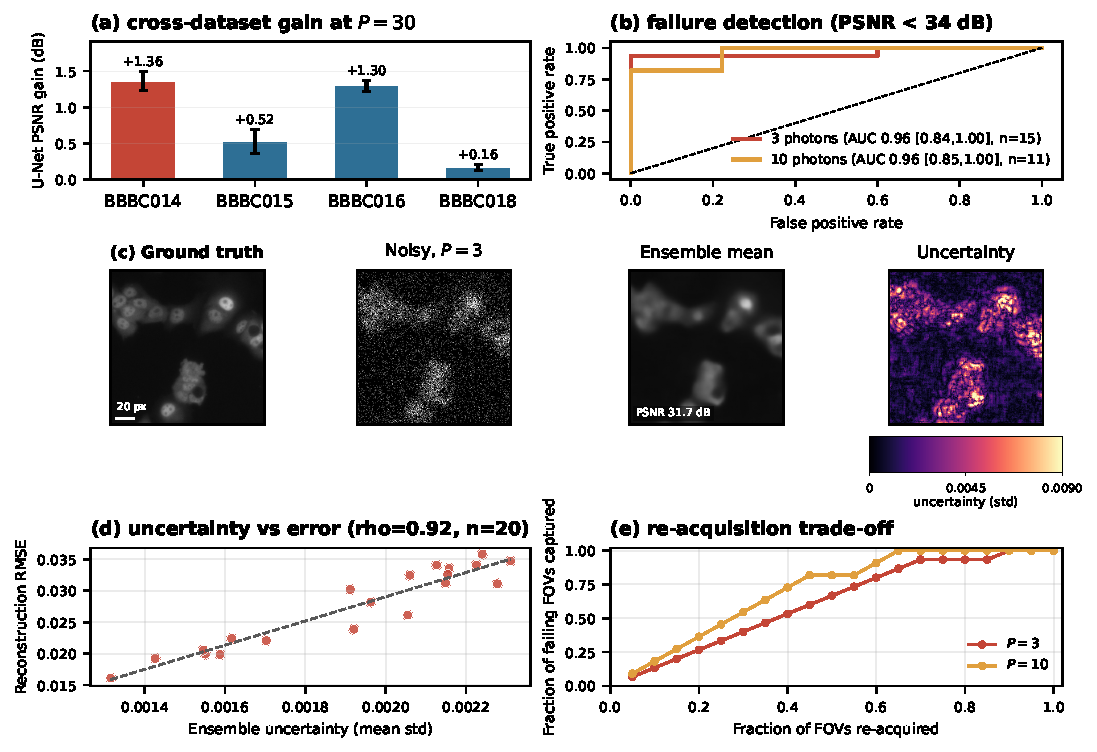
\includegraphics[width=\linewidth]{fig3_cross_uncertainty.pdf}
\caption{(a) 30 光子时混合剂量网络相对调好的 TV 反卷积在四个数据集上的平均 PSNR 增益；红色为域内，蓝色为外部；误差棒为 95\% bootstrap CI，外部 TV 权重按数据集在 5 个单独 field 上调参。(b) 基预算不确定度 ensemble 的失败检测 ROC。(c) $P=3$ 时验证 FOV 的例子：真值、噪声输入、ensemble 均值和不确定度（标准差）。(d) held-out FOV 上不确定度与 RMSE，带线性拟合。(e) 重采集权衡：捕获的失败 FOV 比例对重采集 FOV 比例，$P=3$ 和 10。AUC 和 95\% bootstrap CI 在 (b)；30 光子只有一个 FOV 失败，不显示 AUC。}
\label{fig:cross}
\end{figure}

\subsection{不确定度识别不可靠视野}
三模型 ensemble 给出逐像素不确定度图（图~\ref{fig:cross}c）。$P=3$ 时不确定度集中在细胞边界和暗结构，误差最大处也在此。跨 FOV，不确定度与重建 RMSE 相关（Spearman $\rho=\RhoThree$），并把低于 34\,dB 的失败 FOV 与成功 FOV 分开，$P=3$ 时 AUC \AucThree（95\% CI 0.84--1.00），10 光子时 \AucTen（0.85--1.00）（图~\ref{fig:cross}b,e；SI S4）。30 光子时只有 \NFailThirty\ 个 FOV 低于目标，因此不报告 AUC。这提供了一个实用的质量控制信号：高不确定度的场可以重采或保守解释，而不需要真值图。

\subsection{真实噪声/干净数据}
为了检验恢复增益能否在真实噪声上成立，我们在 AI4Life-MDC25 的 1{,}951 个真实噪声/干净对上训练相同 U-Net 拓扑（48 通道），在 \RealN\ 个 held-out 对上评估（图~\ref{fig:real}、表~\ref{tab:real}）。网络达到 \RealUnetP\,dB PSNR 和 \RealUnetS\ SSIM，对比 affine 校准 BM3D \RealBMThreeP\,dB/\RealBMThreeS、NLM \RealNlmP\,dB/\RealNlmS、TV 去噪 \RealTvP\,dB/\RealTvS，以及噪声输入 \RealNoisyP\,dB。BM3D 与 NLM 相差 0.05\,dB 以内；网络相对 BM3D 的配对增益为 \RealGain\,dB（95\% CI \RealCI；精确 Wilcoxon $p=\RealPvalue$），相对 NLM \RealGainNlm\,dB，相对 TV 去噪 \RealGainTv\,dB；在 \RealN\ 对中赢 \RealWins\ 对。预算匹配的 DnCNN（相同 16k patch、80 epoch）达到 \RealDncnnP\,dB/\RealDncnnS，比 affine BM3D 高 \RealDncnnGain\,dB，只比 U-Net 低 \RealUnetGainDncnn\,dB（95\% CI \RealUnetDncnnCI；\RealUnetDncnnWins/243）。因此，相对经典方法的增益不是某一个深度架构特有的，U-Net 只保留很小的优势。这是一个同源真实噪声结果：训练和测试对来自同一采集协议，field 不重叠，也没有近重复图像；真实对不含模糊，因此验证的是匹配协议内的去噪，而不是去模糊。

FMD 额外在预先指定的 301 个 held-out field 中的 150 个上评估（SI S7b）。使用按显微镜调参的基线，U-Net 达到 \FmdUnetP\,dB/\FmdUnetS\ SSIM，对比 BM3D \FmdBMThreeP\,dB/\FmdBMThreeS（+\FmdGain\,dB，\FmdWins/\FmdN）。这些数字没有做 affine 校准，因此 FMD 仍是次要的上界检查，不作为 headline；主要真实证据是上面的细胞核数据。

同一训练模型应用到同一 release 的 20 个大幅 BBBC006 field 时，排序反转：网络 \LargeRealUnetP\,dB，低于原始经典基线 BM3D \LargeRealBMThreeP\,dB、NLM \LargeRealNlmP\,dB 和 TV \LargeRealTvP\,dB。大幅场有 16-bit 饱和参考和不同的噪声模型，因此这是跨来源迁移失败，而不是对同源结果的否定。它说明训练和部署采集匹配仍然必要，也是我们把剂量扫描描述为受控模拟、而不是真实低剂量验证的主要原因。

\begin{table}[H]
\centering
\caption{AI4Life-MDC25（Jacquemet 来源）的真实噪声/干净对。\RealN\ 个 held-out 细胞核 field；经典参数在验证 field 上调参并做 affine 校准；DnCNN 是第二个监督深度基线。PSNR 单位为 dB。}
\label{tab:real}
\begin{tabular}{lcc}
\toprule
方法 & PSNR（dB） & SSIM \\
\midrule
\multicolumn{3}{l}{\emph{AI4Life 细胞核，\RealN\ 个 held-out field}} \\
噪声输入 & \RealNoisyP & \RealNoisyS \\
TV 去噪 & \RealTvP & \RealTvS \\
NLM & \RealNlmP & \RealNlmS \\
BM3D & \RealBMThreeP & \RealBMThreeS \\
DnCNN（监督） & \RealDncnnP & \RealDncnnS \\
U-Net & \RealUnetP & \RealUnetS \\
\bottomrule
\end{tabular}

\end{table}

\begin{figure}[H]
\centering
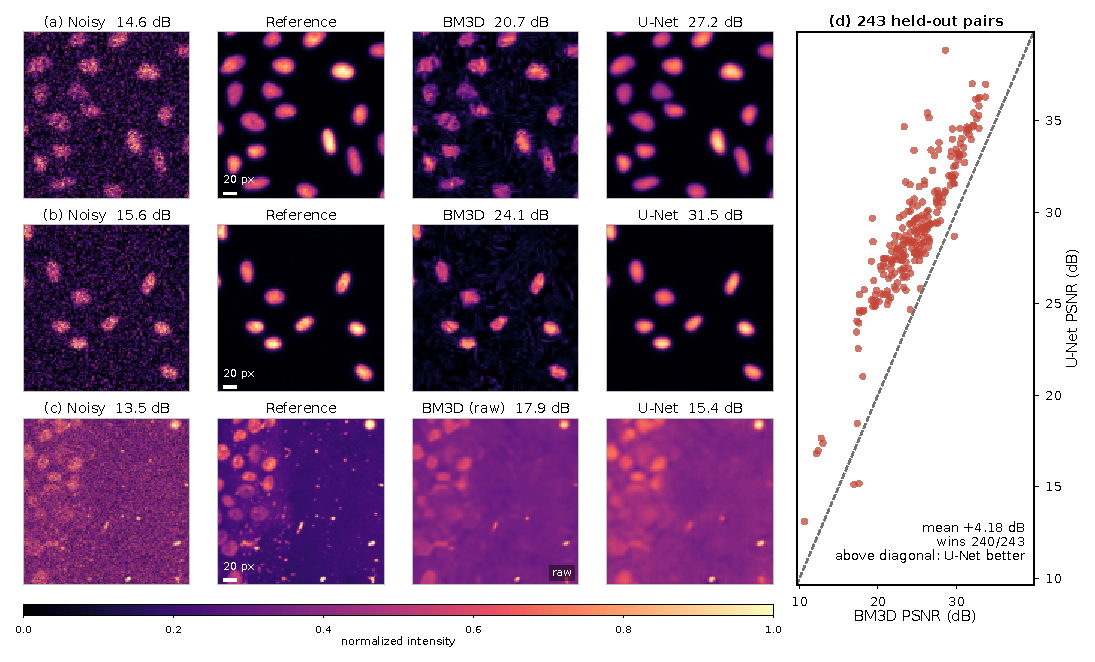
\includegraphics[width=\linewidth]{fig4_real.pdf}
\caption{held-out AI4Life-MDC25 对上的真实数据验证。(a,b) 按 U-Net PSNR 的 25th 和 75th 百分位选取的两个固定 held-out 对（中位质量示例，不是挑最好的），显示噪声输入、干净参考、affine 校准 BM3D、U-Net；数字是单对 PSNR。(c) 同一 release 的一个大幅 BBBC006 field（固定 field 和裁剪），同一权重在跨来源迁移下失败；此处 BM3D 为原始输出，面板内标为 raw。(d) \RealN\ 个 held-out 对的 U-Net 对 BM3D 逐对 PSNR；虚线为 $y=x$，有 \RealWins/\RealN\ 对在对角线上方。所有图像共用一个 $[0,1]$ 归一化强度色条；比例尺 20 像素。}
\label{fig:real}
\end{figure}

\subsection{对照、PSF 鲁棒性与速度}
与 64 通道/48k/150 预算相同的相位打乱对照，使用同功率谱但没有空间结构的替代图像训练，在 $P=3,30,100$ 达到 \ScrPthree、\ScrPthirty、\ScrPonehundred\,dB，低于真实模型（\UNetPthree、\UNetPthirty、\UNetPonehundred）和 TV 反卷积（\DecPthree、\DecPthirty、\DecPonehundred；SI）。因此，相对经典基线的增益需要学到的样本结构，而不只是额外的去噪容量。

混合剂量模型能容忍适度的高斯宽度失配：30 光子时，$\sigma=1.5,2.0,2.5$ 分别达到 \SigmaUPfifteen、\SigmaUPtwo、\SigmaUPtwopfive\,dB，对比同 $\lambda=0.04$ 的 TV 反卷积 \SigmaDecfifteen、\SigmaDectwo、\SigmaDectwopfive\,dB；网络在三个宽度上分别领先 1.07、1.36、1.00\,dB。但高斯训练的模型不能迁移到形状和宽度都不同的 PSF：用 in-focus Airy PSF（NA 1.4、520\,nm、100\,nm 像素；FWHM 约 1.9 像素，比 $\sigma=2$ 的训练核窄）时，它在 $P=3/30/300$ 只达到 \AiryStrongUThree、\AiryStrongUThirty、\AiryStrongUThreeHundred\,dB，即相对使用正确 PSF 的 TV 反卷积 \AiryStrongGainThree、\AiryStrongGainThirty、\AiryStrongGainThreeHundred\,dB。用 50/50 高斯/Airy 混合训练的模型恢复了高剂量性能：\AiryUThree、\AiryUThirty、\AiryUThreeHundred\,dB（增益 \AiryGainThree、\AiryGainThirty、\AiryGainThreeHundred\,dB；95\% CI \AiryCIThree、\AiryCIThirty、\AiryCIThreeHundred；20/20 FOV），同时在高斯基准上保持 \PsfMixGaussPThree、\PsfMixGaussPThirty、\PsfMixGaussPThreeHundred\,dB。因此，剂量无关结果并不绑定于精确的高斯核，只要训练分布覆盖部署 PSF。一个探索性的剂量+PSF 条件化模型（32 通道、20k patch、60 epoch；同时输入光子数和 $\sigma$）在同样 $\sigma$ 下达到 36.69、36.03、35.44\,dB，比强盲模型低 0.23--0.67\,dB；由于它既不是预算匹配也不是盲的，我们不采用（\texttt{results/dscond\_eval.json}）。在 30 光子时加入标准差 0.005 或 0.01（1.3 或 2.6 个 8-bit 计数）的高斯读出噪声，网络和公平 TV 的变化都不超过 0.04\,dB（SI）。

推理在 A100 上每个 $128\times128$ patch 需 \SpeedGPU\,ms，在单 CPU 核上需 \SpeedCPU\,ms；30 次 ADMM TV 反卷积在单 CPU 核上需 \SpeedTV\,ms。因此网络在同一 CPU 核上快 \SpeedFactorCPU$\times$，在 GPU 上快 \SpeedFactorGPU$\times$。完整 $1360\times1024$ FOV 约需 85 个 patch，即 GPU 上约 0.1\,s 或单 CPU 核上约 2.5\,s；这支持交互式和许多在线流程，但不支持单 CPU 核上的全 FOV 帧率反馈。

\subsection{自适应分配依赖目标}
我们还测试了用廉价预览和逐 FOV 不确定度来为每个场选择不同剂量。一个能访问每个 FOV 完整剂量响应的 oracle 在测试目标上可省 42--71\% 光子，但在验证 FOV 上校准的无真值策略在匹配测试成功率时不能稳定超过最佳固定剂量；细节在 SI。因此我们建议使用图~\ref{fig:dose}e 读出的固定协议剂量，而不是逐 FOV 分配。

\section{讨论}
增益有两个来源。去噪容量解释了一部分，但相位打乱对照表明，仅靠容量并不能超过公平 TV 反卷积。其余来自对样本结构的先验：$P=3$ 时输入只保留了细胞的位置和大体形状，网络却恢复了 TV 反卷积抹掉的边界和内部纹理；同样的先验在高剂量下提高了可达质量，因为经典方法已经饱和。剂量条件化和专家比较表明，这个先验可以从混合剂量中学到，不需要剂量输入；推理时不需要光子数。与此一致，简单图像统计上的线性探针以 97.9\% 准确率识别五个剂量（小 CNN 为 100\%；SI S8），说明适应有效正则化所需的信息已经在含噪输入中。

使用验证集选择剂量时，协议在四个目标上省 3--3.3 倍光子，三个目标平局；两个验证选择不满足 held-out 准则，而 test-oracle 上界是五项节省、四项平局。SSIM 0.85 时经典方法已经在同一剂量，因此那里的优势是质量上限而不是阈值。跨数据集增益说明先验并不绑定于一种细胞类型或染色，只是在训练分布外更小。

\paragraph{模拟的局限。}
噪声是高斯模糊 Poisson 噪声，PSF 已知且空间不变；没有相机读出噪声、背景结构和光学像差。高 SNR 参考本身也是衍射极限的，所以网络去除的是额外的合成高斯模糊，而不是显微镜 PSF；实验检验的是受控模糊下的光子效率，不是未知物体的完整光学重建。PSF 测试覆盖高斯 $\sigma=1.5$--2.5 和 in-focus Airy PSF；PSF 混合模型在 Airy 下保持增益，但任意、像差或深度变化的 PSF 仍未测试。模拟模型在一个数据集上训练，在另外三个上零样本评估；外部增益更小，混合训练可能改善。

\paragraph{真实数据的局限。}
一个下游 BBBC039 细胞核 mask 检查（逐剂量调 TV）只发现很小的 Dice 增益（0.795 对 0.773，$P=1$；SI），所以恢复优势不会自动转化为大的分割增益。真实检查是同源的：在 \RealN\ 个 held-out AI4Life 对上，真实模型比调好的 BM3D 高 \RealGain\,dB，但同一权重在同一 release 的大幅 BBBC006 field 上失败，因为位深、饱和和噪声模型不同。真实成对数据因此支持匹配采集协议内的恢复，而不是跨来源剂量声称。仅用噪声图训练的 label-free J-invariant 变体\cite{batson2019noise2self}在 held-out 集上达到 17.89\,dB，低于调好的 BM3D（21.30\,dB），说明本工作的增益需要成对干净参考。FMD 检查使用预先指定的 150 个 field 分层子集，并要在 FMD 上重训；它不是零样本迁移，而且 FMD 输出没有 affine 校准。

\paragraph{不确定度与幻觉。}
不确定度 ensemble 使用条件化变体；由于条件化只轻微改变精度，我们预计校准可以迁移，但没有直接检验。学习恢复可能产生看似合理但错误的结构\cite{blau2018perception}；不确定度能标记不可靠场，但不能证明一个自信重建没有伪影。在匹配的真实低剂量数据上验证仍然是定量生物使用前的必要步骤。

最接近的工作在机制和证据上不同。FFDNet 对去噪网络做噪声水平条件化，CARE 学习成对图像的监督恢复映射。这里单个混合剂量模型既不需要噪声水平输入，也不需要逐剂量重训，而且与条件化变体只差 0.05\,dB。Ye 等\cite{ye2025uncertainty}用不确定度驱动自适应重扫描；我们的协议是固定宽场采集，自适应扩展作为负结果放在 SI。Liu 等\cite{liu2020degeneration}使用基于模型的深度先验，而我们的网络是跨剂量端到端训练；Sheneman 等\cite{sheneman2025nearzero}展示硬件近零光子显微镜，而这里是剂量扫描的受控模拟加同源真实检查。

在操作上，实验室可以在感兴趣的剂量范围训练一次，从协议曲线读出目标成功率对应的固定剂量，并用 ensemble 不确定度标记需要更多光的场。方法不需要改变显微镜，推理不需要光子数元数据；模拟模型在剂量范围上训练一次，真实模型在部署协议的成对图像上训练一次。速度适合在线处理预算。

\section{结论}
一个无光子数输入的混合剂量 U-Net，在 100 倍剂量范围上匹配或超过完全调好的 TV-ADMM 基线，并在匹配成功时把光子数节省约三倍。在真实成对数据上，它相对 affine 校准 BM3D 提升超过 4\,dB，在 243 个场中只输 3 个。增益不是容量效应：剂量条件化只增加不到 \CondStrongDelta\,dB，预算匹配的相位打乱对照仍低于 TV。对固定采集协议，这些结果说明不需要剂量元数据和逐剂量重调，恢复方法应按匹配成功率所需的光子预算来比较。下一步是在真实低剂量采集和其他显微镜 PSF 上做前瞻性验证。

\section*{数据与代码可用性}
所有数据集都是公开的：BBBC014、BBBC015、BBBC016、BBBC018 和 BBBC039 来自 Broad Bioimage Benchmark Collection\cite{ljosa2012bbbc}，AI4Life-MDC25-Nuclei\cite{ai4life_mdc25_2025}（Zenodo 15624741，CC BY 4.0）和 AI4Life-MDC25-FMD\cite{ai4life_mdc25_fmd_2025}（Zenodo 15761900，CC BY 4.0）； accession 号和 license 列在方法中。数据切分、训练、基线、统计和绘图代码，以及 JSON 结果和 checkpoint，将随稿件释放。

\begingroup
\small
\bibliographystyle{unsrt}
\bibliography{references}
\endgroup
\end{document}
